\documentclass[a4paper,twoside]{report}
\usepackage[a4paper, margin=35mm]{geometry}
\usepackage{graphicx}
%\usepackage[T1]{fontenc}
\usepackage{bookmark}
\usepackage{array,booktabs}
\usepackage{lmodern}
\usepackage{float}
\usepackage{multirow,bigdelim}
\usepackage{textcomp}
\usepackage{fancyhdr}
\usepackage{amsmath}
\DeclareMathOperator{\sign}{sign}
\DeclareMathOperator{\argmin}{argmin}
\newcommand{\pvalue}{\mathop{p{\textnormal{-value}}}}
\usepackage{algorithmic,algorithm}
\usepackage{amssymb}
\usepackage{enumitem}
\usepackage{titlepic}
%\renewcommand{\familydefault}{\sfdefault}
\usepackage{tocvsec2}
\usepackage[titletoc]{appendix}
\usepackage[dvipsnames]{xcolor}
\usepackage{tocloft}
\usepackage{csquotes}
\usepackage{rotating}
%\usepackage[round]{natbib}  
\usepackage{color}
\usepackage{hyperref}
\usepackage[acronym,toc,section=section]{glossaries}
\pagestyle{fancy}

\begin{document}
%The next section \ref{statams} shows the derivation of the form in eq. \ref{ams} in the context of $\pvalue$s.
\chapter{Statistical Derivation of the AMS}
\label{statams}

For a classifier $h$ with a selection region $\mathcal{H} = \{\mathbf{x}: h(\mathbf{x}) = s\}$, the number of events $n = |\mathcal{H}|$ in the selection region of a classifier follows a Poisson distribution as its mean can be expressed by the sum of two Poisson random variables $\mu_b + \mu_s$, where $\mu_b$  is the expected number of background events in the selection region and $\mu_s$ is the expected number of signal events in the selection region. 

A Poisson probability for $n$ events with an average rate of occurrence of $\mu_{b} + \mu_{s}$ is given by,

\begin{equation}
P(n \vert \mu_{b},\mu_{s}) = \frac{(\mu_{b} + \mu_{s})^{n}}{n!}e^{-(\mu_{b} + \mu_{s})}
\end{equation}

%\begin{figure}[h]
%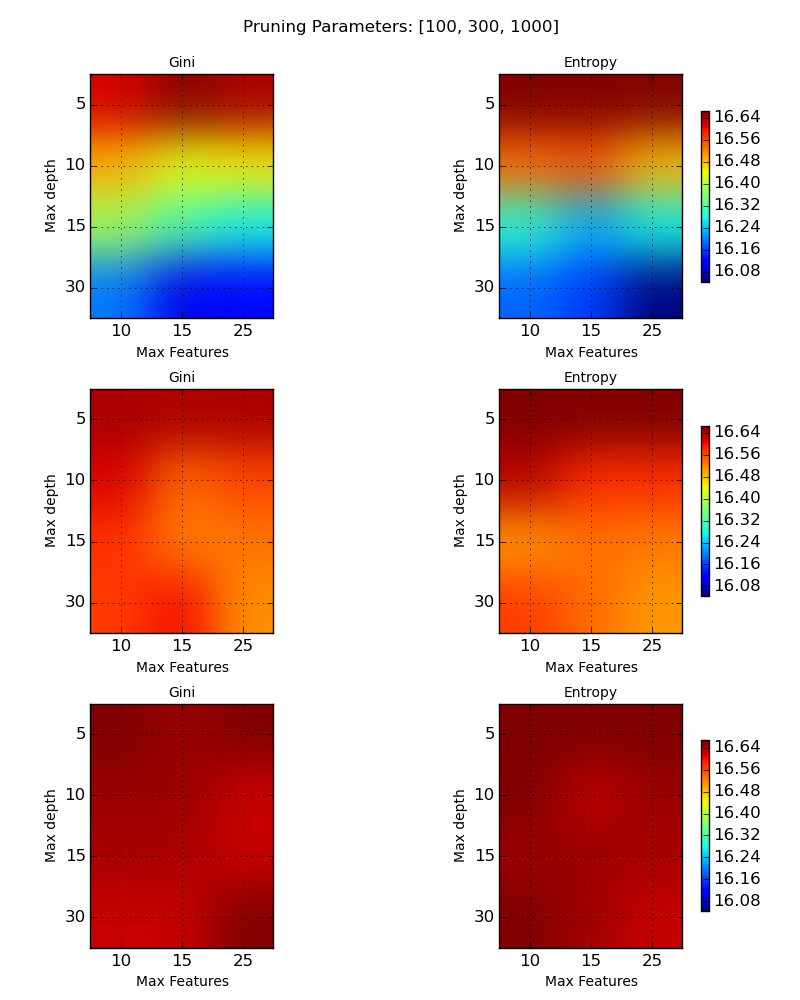
\includegraphics[width=\textwidth]{images/Grid_error_gini_entropy.png}
%\caption{Density of the balanced classification error for different pruning parameters which refer to the minimum number of leaves required to split a node and the minimum number of leaves required to qualify as a leaf.}
%\label{gini}
%\end{figure}

The null hypothesis we are testing for is $H_{0}: \mu_{s} = 0$ and the alternative hypothesis is $H_{1}: \mu_{s} > 0$. We compute the likelihood ratio defined as, 

\begin{equation}
\Lambda = \frac{P(n \vert 0,\mu_{b})}{P(n \vert \mu_{s},\mu_{b})} = \Big( \frac{\mu_{b}}{\mu_{s} + \mu_{b}}\Big)^{n}e^{\mu_s} = \Big( \frac{\mu_{b}}{n}\Big)^{n}e^{n - \mu_{b}}
\end{equation}

where $\mu_s = n - \mu_b$ is the maximum likelihood estimator for $\mu_s$. Next, we need the sampling distribution of the test statistic $\Lambda$ to derive a $\pvalue$. 

By Wilk's theorem the test statistic $-2\ln(\Lambda)$ follows a $\chi^{2}$ distribution in the large sample limit as $n \rightarrow \infty$. This means that we can compute likelihood $\Lambda$ and use the statistic $-2\ln(\Lambda)$ under a $\chi^{2}$ cumulative distribution function to compute the $\pvalue$. 

\begin{equation}
p = 1 - Q(-2\ln(\Lambda))
\end{equation}

Q is the $\chi{2}$ cumulative distribution function.

The test statistic, 

\begin{equation}
q_{0} = \begin{cases} -2\ln(\Lambda),  \textrm{   }n > \mu_{b}\\ 0,  \hspace{11mm} \textrm{otherwise }
\end{cases}
\end{equation}

serves as the basis of the statistical test. In order to see why, a significant upward fluctuation in the data constitutes evidence that a background only hypothesis ($\mu_s = 0$) is not supported in the data. Thus, higher values of the test statistic - $q_{0}$ point to increasing evidence of incompatibility with the null hypothesis. If the data fluctuates downward such that one finds events fewer than that expected by the background process then this also points to incompatibility with the null but not because of presence of signal events but rather some other systematic error hence in this case we assign $q_{0} = 0$.

\begin{figure}
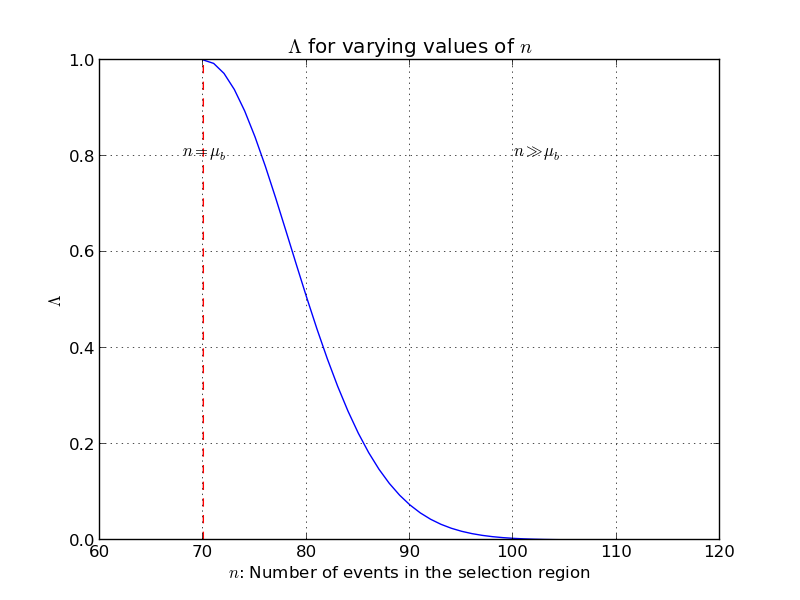
\includegraphics[scale=0.6]{images/lambda.png}
\end{figure}

\begin{figure}
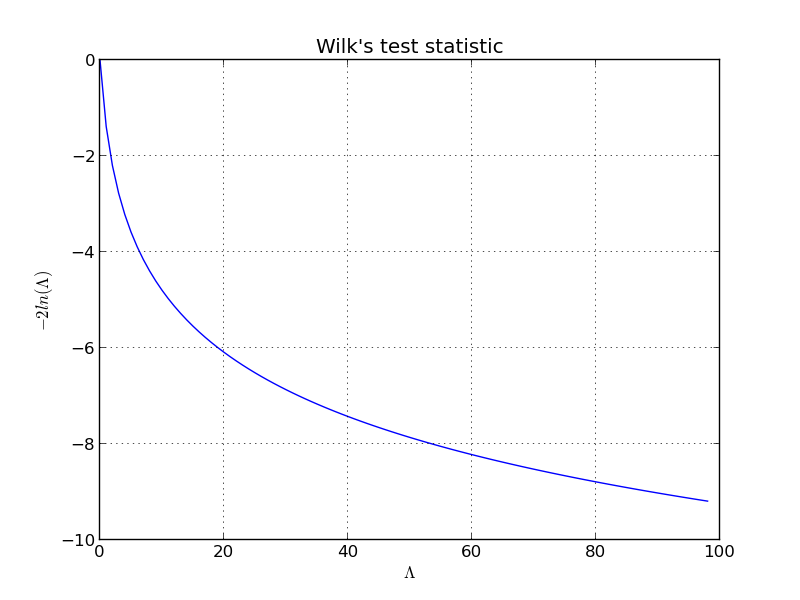
\includegraphics[scale=0.6]{images/wilks.png}
\end{figure}

Next, we need to define the pdf (probability density function) of $q_{0}$. Note that $q_{0}$ when $n > \mu_{b}$ follows a $\chi^{2}$ distribution in the large sample limit. The pdf of a $\chi^{2}$ distribution is, 

\begin{equation}
\dfrac{1}{2^{\frac{k}{2}}\Gamma(\frac{k}{2})}x^{\frac{k}{2} - 1}e^{-\frac{x}{2}}
\end{equation}

where $k$ is the degrees of freedom (since a $\chi^{2}$ random variable is the sum of $k$ independent standard normal variables. If $Z_{1},...,Z_{k}$ are standard normal then, $Q = \sum_{i=1}^{k}Z_{i}^{2}$ is $\chi^{2}$ distributed with $k$ degrees of freedom) and $\Gamma$ is the gamma function, $\Gamma(n) = (n-1)!$

Using the pdf of the $\chi^{2}$ distribution and the fact that $k = 1$ for $q_{0}$ and $\Gamma\bigg(\dfrac{1}{2}\bigg) = \sqrt{\pi}$ we deduce that the pdf of $q_{0}$ is,

\begin{equation}
f(q_{0}) = \frac{1}{2}\delta(q_{0}) + \frac{1}{2}\frac{1}{\sqrt{2\pi}}\frac{1}{\sqrt{q_{0}}}e^{-\frac{q_{0}}{2}}
\end{equation}

where $\delta$ is the Dirac delta function and we use the result that when a random variable takes $n$ discrete values $x_{1},...,x_{n}$ with associated probabilities $p_{1},...,p_{n}$ the probability density function is,

\begin{equation}
f(t) = \sum_{i=1}^{n}p_{i}\delta(t-x_{i})
\end{equation}

The cumulative distribution function of $q_{0}$ is,

\begin{equation}
F(q_{0}) = \Phi(\sqrt{q_{0}})
\label{cum}
\end{equation}
where $\Phi$ is the cumulative distribution function (cdf) of the standard normal variable. 

To derive this from first principles consider the expression of the cdf of the random variable $q_{0}$ as defined above,

\begin{equation*}
\begin{aligned}
F_{q_{0}}(x) &= \int_{-\infty}^{x}f_{q_{0}}(t)dt\\
& = \frac{1}{2}\int_{-\infty}^{x} \delta(t)dt + \frac{1}{2}\frac{1}{\sqrt{2\pi}}\int_{-\infty}^{x}\frac{1}{\sqrt{t}}e^{-t/2}dt\\
&= \frac{1}{2}\bigg[1 + \textrm{erf}\bigg(\sqrt{\frac{x}{2}}\bigg) \bigg] \\
&= \Phi(\sqrt{x})
\end{aligned}
\end{equation*}
where erf($\bullet$) is the gaussian error function defined as,

\begin{equation*}
\textrm{erf}(x) = \frac{1}{\sqrt{\pi}}\int_{-x}^{x}e^{-t^{2}} dt
\end{equation*}

This is closely related to the standard normal cumulative distribution function through, 

\begin{equation*}
\Phi(x) = \frac{1}{2}\bigg[1 + \textrm{erf}\bigg(\frac{x}{\sqrt{2}}\bigg)\bigg]
\end{equation*} 
and

\begin{equation*}
\Phi(x) = \int_{-\infty}^{x}e^{-t^{2}/2}dt
\end{equation*}

The $\pvalue$ and significance is from eq. \ref{cum} is therefore,

\begin{equation*}
p = 1 - \Phi(\sqrt{q_{0}}) 
\end{equation*}

\begin{equation*}
Z = \Phi^{-1}(1-p)
\end{equation*}

This leads to the result,

\begin{equation}
Z = \sqrt{q_{0}} = \sqrt{2\Bigg( n\ln\bigg(\frac{n}{\mu_{b}}\bigg) - n + \mu_{b}\Bigg)} 
\end{equation}

if $n > \mu_b$ and Z = 0 otherwise. The quantity Z measures significance in terms of units of sigmas from the mean, a Z value of 5 would correspond to a 5$\sigma$ effect and in physics is regarded as necessary to claim a discovery of a new particle.

\end{document}